\chapter{Point Cloud command}
\label{Chap:PointCloud}


%-----------------------------------------------------------------------
%-----------------------------------------------------------------------
%-----------------------------------------------------------------------

\section{Generalities}

%-----------------------------------------------------------------------
\subsection{Introduction}

This section introduce some command/piece of code that have been devlopped for simulating
images and depth map from lidar data.  This simulation was done with the ambition of being usable as
training data set for computing canopy model from photogrammetric acquisition. This
simulation pretend by no way to be physically based, the assumption behind this simulation
is that what make the canopy difficult to modelize in photgrammetry is its 3D structure that :

\begin{itemize}
   \item make it difficult to modelize (for ex via regularization);
   \item generate highly variable images for small change of point of view.
\end{itemize}


So the pitch of this simulation is that, if we create data that reflect this difficulties, 
we will able to train the networks.  Possibly, the images that we will be generated are "more
challenging" that  real images, but be we hope that being a "too tough teacher with a network" is not a problem.

Conversely, a postive point of simulation is that we can generate "perfectly" registered data.



%-----------------------------------------------------------------------
\subsection{MMVII format}

As at this step, it is just a \emph{quick and dirty} prototype, this means that the
devlopment has been made with the objective of minizing the effort for what
was projected and absolutlely no idea of long term maintenance and evolution.
For example, we did not  think it 
was pertinent to add "big" librairies for lidar data reading and manipulation.
The code is then based on internal classes and format.

The class for representing a point cloud is {\tt cPointCloud}, it contains essentially:

\begin{itemize}
  \item  a vector of $3d$ point
  \item different optionnal vector, that are attributes of the point
  \item  some information useful for computation as : bounding boxes , offset of point,
         or dynamic of layer \dots
\end{itemize}

For saving and reading  {\tt cPointCloud}, we use {\tt MMVII} facilitie of
automated serialization.  As it's very huge data , we use the binary
format that generate {\tt ".dmp"} files.

At the time being, we  dont make any effort for maintening historical compatibility
of this format.  It will probably evolve with new layer, and at each evolution
previous file may become unusable 
 Of course, at longer term, if this devlopment
continue, we will change that by : make an evolutive format or adopt a standard format.
 (by the way,  the format already includes some layer for handling backward compatibility).

%-----------------------------------------------------------------------
%-----------------------------------------------------------------------
%-----------------------------------------------------------------------

\section{Create and viusualizng}


%-----------------------------------------------------------------------

\section{Import   data with  {\tt ImportTxtCloud}}

We can only import  data in ply text format.  More precisely , {\tt MMVII} use the general facilities
for parsing text file with identical line structure, and do not interpret the ply "semantic". Any text format
close enough to ply, would be readable.

Example of use :

\begin{verbatim}
 MMVII ImportTxtCloud 18355_51565.ply "XYZBla" NumL0=30O OffsetIsP0=true Bytes8=false HELP
\end{verbatim}

This command will generate a file {\tt 18355\_51565.dmp}.
In this command :

\begin{itemize}
   \item {\tt "XYZBla"}  means that we will read the 3 coordinates at the begining of each line and skip after
   \item {\tt NumL0=30O}  skip the first lines , probably $300$ is "too much", the important is to skip all the header ;
   \item {\tt Bytes8=false }  mean that the coordinate are store on $4$ byte (and not $8$);
   \item {\tt  OffsetIsP0=true }  mean that the coordinate are store with an offset, and that thi offset is computed
         from first point, this is often required with geographic coordinates to maintain sufficient accuracy.
\end{itemize}

Note that this import, can be quite long .

{\bf To be done : import ply binary format}.

%-----------------------------------------------------------------------

\section{Cliping data with  {\tt CloudMMVIIClip}}

It is often convenient to make test on small point cloud.  For this one can use the
command {\tt CloudMMVIIClip} :


\begin{verbatim}
MMVII CloudMMVIIClip 18355_51565.dmp [0.4,0.4,0.6,0.6]
\end{verbatim}

The command will generate a file {\tt  Clip\_18355\_51565.dmp}.  Note that the box is relative to the global
box (that is stored in the file).


%-----------------------------------------------------------------------

\section{Visualizing data with {\tt CloudMMVII2Ply}}

As the format {\tt ".dmp"} is purely internal, it cannot be visualized with standard tool.
This is why it possible to create ply version of {\tt dmp} files with the command 
{\tt CloudMMVII2Ply}.  This is specially usefull with colored point cloud
(see~\ref{Cloud::Colorate}).

The command is pretty basic and obvious , for example: 

\begin{verbatim}
MMVII CloudMMVII2Ply Clip_18355_51565.dmp
\end{verbatim}

%-----------------------------------------------------------------------
%-----------------------------------------------------------------------
%-----------------------------------------------------------------------

\section{Colouring point cloud with {\tt CloudMMVIIColorate}}

\label{Cloud::Colorate}


Before generating image, we must compute the "colour" of each point/leave. The hypothesis
we do for this are the following :


\begin{itemize}
   \item the colour of each leave depend only of the quantity of light/energy it receive taking into account occlusions;
         this model is quite simplist because in real tree each leave has a different intrisic
         colour (albedo) , but we adpot it because :
         \begin{itemize}
              \item  our intution when observing real tree is that the light occlusion is predominant over the albedo
                     variation for explaining contrats in images (except maybe trees at the begining of automn, 
                     when there is a mix of green \& brown leaves)
              \item  we have no mean to generate realistic albedo varaiation;
              \item  ometting albedo variation make the problem rather more difficult, and in the doubt, it's better
                     to train the networks with data too difficult than to easy.
         \end{itemize}

         by the way, we dont exclude to add later some randomized albedo or use the lidar  intensity when it exist
         to complement the previous value.


   \item the light is made from $2$ sources : an homogeneous halph sphere corresponding to the \emph{"sky"} and a mono directionnal spot light 
         corresponding to the \emph{"sun"}

   \item leaves are spheres.

\end{itemize}


The command is {\tt CloudMMVIIColorate} it takes a {\tt MMVII} cloud point as input and create a new a {\tt MMVII} cloud point.
Let's describe a few optional parameters :

\begin{itemize}
   \item  {\bf NbSampS} control the  number sampling of the sphere,  more précisely each face
         of cube generate $NbSampS*NbSampS$ direction ;

   \item {\bf Sun}  possibly add "high" energy cooressponding  to  a direction (direction of the sun), it's a 3d point,
         let $Sun=[T,P,W]$  , the direction is a point of spherical coordinate $\theta = T * \frac{\pi}{2}$ and
        $\phi = \frac{\pi}{2} + P$  ;  for $W$ it's the weithing of the sun compared to the total energy brought by the 
        other direction .
\end{itemize}

Note that it's that use of {\bf Sun} parameter in this command, is only usefull for visuaslizing point cloud
in $3d$  with  {\tt CloudMMVII2Ply}.  For generation of images in sections \ref{Cloud:Epip} and  \ref{Cloud:MultiV}
, we recommand rather to add the sun at each image generation (because adding one direction take a few part
of computing time).


%-----------------------------------------------------------------------
%-----------------------------------------------------------------------
%-----------------------------------------------------------------------

\section{Training data sets for epipolar with {\tt CloudMMVII\_GT\_EpipOrthoC}}

\label{Cloud:Epip}


The command  {\tt CloudMMVII\_GT\_EpipOrthoC}  generate a set images corresponding
to orthographic projections that are all in epipolar correspondance. The direction
of projection are all on the same circle passing through vertical and regularly 
distributed. The command take $2$ mandatory parameters,
a {\tt MMVII} point-cloud, and a vector $V$ of $3$ to $5$ real value  controling
the direction of projection :

\begin{itemize}
   \item  $V_0$  is such that $V_0 * \frac{\pi}{2}$ is the common longitude of the direction  of projection ;
   \item   $V_1$ is the such there   $1+2*V_1$ projections;
   \item   $V_2$ is such that  $ \frac{\pi}{2}+V_2$ is the longitude of  the first direction;
   \item   $V_3$ is such that  $ \frac{\pi}{2}+V_3$ is the longitude of  the last direction, by default $V_3 = - V_2$ ;
\end{itemize}


The programm generate  results in the folder {\tt MVII-PhgrProj/VISU/CloudMMVII\_GT\_EpipOrthoC} . These
result contains :

\begin{itemize}
   \item the "radiometric" simulated images ;

   \item  ground truth disparities,  by default they are generated for consecutive directions and
          in both way, but this can be changed with optional parameter {\tt DeltaPax}
   
   \item weighting image proportional to the density of point that have been projected, it can be used
         to generate mask for no data image;

\end{itemize}

A \emph{sun} can be added like in \ref{Cloud::Colorate}. The images of figure~\ref{PC:Simul:Epip}
were generated with the following command.

\begin{verbatim}
MMVII CloudMMVII_GT_EpipOrthoC Col-Clip-Leave2-2.dmp "[0.0,2,0.25]" "Sun=[-0.5,0.5,2]" SaveImD=1 Show=1 
\end{verbatim}


\begin{figure}
\centering
        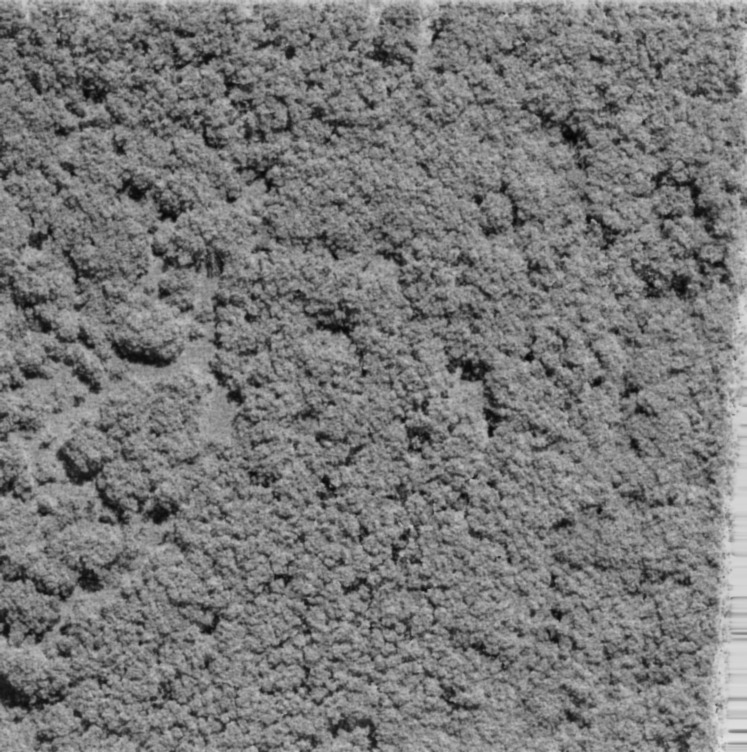
\includegraphics[width=4cm]{CommandReferences/ImagesComRef/Rad0.jpg}
        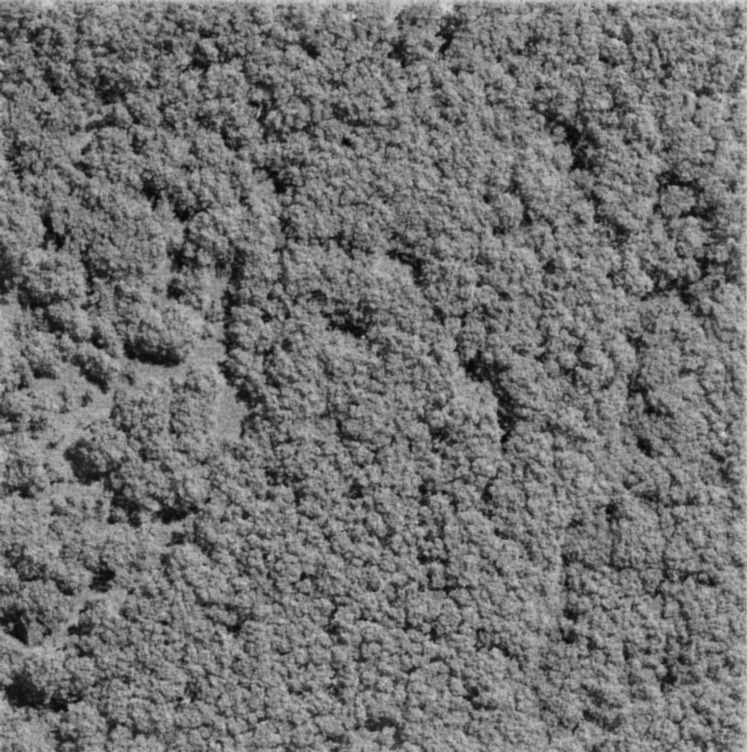
\includegraphics[width=4cm]{CommandReferences/ImagesComRef/Rad1.jpg}
        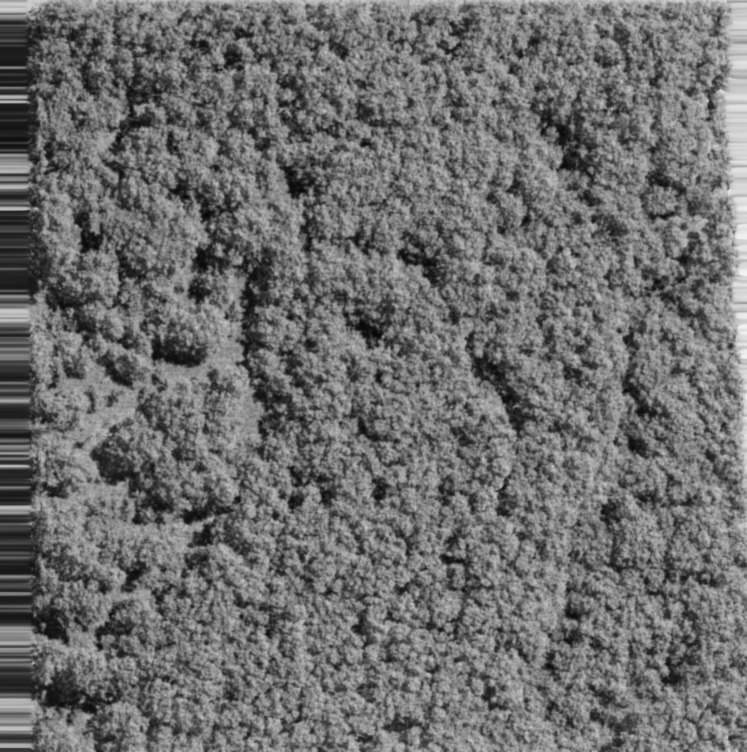
\includegraphics[width=4cm]{CommandReferences/ImagesComRef/Rad2.jpg}
        \caption{Example of radiometric images simulated}
\label{PC:Simul:Epip}
\end{figure}


%-----------------------------------------------------------------------
%-----------------------------------------------------------------------
%-----------------------------------------------------------------------

\section{Training data sets for multi viewwith {\tt CloudMMVII\_GT\_MultiView}}


\label{Cloud:MultiV}

For multiview, we can use the {\tt CloudMMVII\_GT\_MultiView}. It take $3$ parameters :

\begin{itemize}
  \item input point cloud;
  \item size of images
  \item a folder for output cameras \emph{and} images  (to be changed maybe later, dont know where to put it ...)
\end{itemize}

The images are generated with a conical projection, the field of view of the camera can be controled
with optionnale parameter {\tt FOV}, the number of images can be controled with parameter {\tt Overlap},
the image are generated if at least $50\%$ are inside the box (can be changed with parameter {\tt MinInside}).





